\section{Introduction}\label{sec:intro}
Producing reward signal is a fundamental brain function for animals to live and reproduce. Positive rewards such as pleasure encourages us to eat and find partners, while negative rewards such as fatigue help us protect ourselves. These reward signals affect our behavior through learning. Our brain produce reward signal to a certain stimulus such as good food, and the signal is used to reinforce our behavior that lead to the reward. This mechanism is called reinforcement learning (RL) and has been extensively studied in both neuroscience and computer science. Neuroscientists have revealed that our brain has some hot or cold spots that respond to good or bad events~\citep{berridgeAffectiveNeurosciencePleasure2008}, and how those signals are used for learning~\citep{schultzNeuronalRewardDecision2015}, while computational reinforcement learning has provided theoretical models and several applications including game-playing agents and robotics~\citep{suttonReinforcementLearningIntroduction2018}.

% Problem: Reward evolution
% Why this topic has been underexplored, and how we can find some interesting points from this line of research
Due to its significant contribution to our lives, how our reward system have evolved is an interesting open question. A common explanation is based on natural selection, arguing that rewards have evolved to help animals survive in the environment and successfully reproduce offspring (e.g., by~\cite{schultzNeuronalRewardDecision2015}). This hypothesis sounds reasonable, because our reward functions such as one for food reward are actually helping us to live longer and contribute to our fitness. However, there remain some questions in the detailed process of reward evolution. Given that some animals, including ascidians, have evolved to have evolved to abandon brain, the conditions under which reward system is required is not obvious. Another question is how the mechanism for suppressing rewards evolved. For example, rewards for food are suppressed by satiety. It is not obvious how such suppression mechanisms have evolved along with rewards.

% Importance of simulation
While biological studies on both evolutionary biology and neuroscience are highly important to address these questions, we argue that computational study can also contribute to this area by providing a simplified model of real evolution. A good example is the relationship between biological and computational RL, which have evolved closely. While computational RL has provided us with useful engineering techniques, it has also provided a promising computational model for how animals learn. We aim to make a similar contribution to the problem of reward evolution.

% Why population-based model is important
For this purpose, what kind of simulation model is suitable? Natural selection is the idea that genetic traits that contribute to more offspring will survive and evolve. Indicators such as the average number of births that assess this reproductive success are also called fitness. Some classical studies on the evolution of learning \citep{hintonHowLearningCan1987} have conducted simulations by explicitly designing a fitness function for a particular task. This approach has an advantage that evaluation of genetic traits is computational cheap, whereas to evaluate genetic traits from reproductive success alone would require simulations over several generations in a given population. However, this method has a disadvantage that the design of the fitness function is not always natural because of the designer's bias. Since we are interested in how biologically plausible rewards evolve, we prefer to use more natural measures such as reproductive success. Furthermore, today, we have much greater computational resources that enable larger populations are possible.

% Proposed simulation model
To this end, we propose to use a distributed evolutionary model of reward function, inspired by the concept posed by embodied evolution (EE)~\cite{watsonEmbodiedEvolutionDistributing2002}. While a major line of work in evolutionary computation considers evolution with a designed fitness function, EE aims to simulate evolution in a fully distributed way with particular death and birth conditions.

an ecologically-plausible environment to conduct simulation.

% Result

\section{Related Work}\label{sec:related}
RL community has contributed to \citet{singhWhereRewardsCome} is also important.

Therefore, \citet{watsonEmbodiedEvolutionDistributing2002} proposed a scheme called embodied evolution (EE). In EE, all the evaluation, reproduction, and selection are performed by individual robots in a decentralized manner, while traditional ER employs a centralized selection similar to GA\@. Robots die based on a defined lifespan and mortality rate, and newly born ones replace the programs of the dead robots.

The series of studies by \citet{elfwingBiologicallyInspiredEmbodied2005,elfwingDarwinianEmbodiedEvolution2011a,elfwingEmergencePolymorphicMating2014} drew the main inspiration to this work.
They tried to evolve shaping rewards and meta parameters of reinforcement learning agents using mobile robots called Cyber Rodents. In particular, \citet{elfwingDarwinianEmbodiedEvolution2011a} evolved reward-shaping parameters of RL agents, showing that rewards that make learning easier had evolved, while \citet{elfwingEmergencePolymorphicMating2014} evolved agents with a hierarchical RL mechanism, where the higher module chooses either foraging or mating, and the lower module outputs more primitive actions. They evolved only the higher decision-making parameters, while the lower modules were learned by RL. In their experiments, they observed two different groups: one that favors mating behavior and the other that favors foraging behavior. In our study, we try to evolve primary rewards instead of shaping rewards or the hierarchical decision-making mechanism they use. \citet{uchibeFindingIntrinsicRewards2008} also experimented with a similar mobile robot where primitive rewards such as food were predefined, but intrinsic rewards such as curiosity were evolved. In contrast, our study attempts to evolve primitive rewards. A drawback of EE is that reproduction is often done by replacing the genome of the same robot \citep{bredecheEmbodiedEvolutionCollective2018}. This makes it challenging to reproduce population increases and decreases by simulation. While the Darwinian EE framework proposed by \citet{elfwingDarwinianEmbodiedEvolution2011a} partially addressed this by having multiple agents as a virtual population inside a robot, we allow for population increase and decrease in simulation.

\section{Simulation Model and Environment}\label{sec:method}

\begin{figure}[t]
  \centering{}
  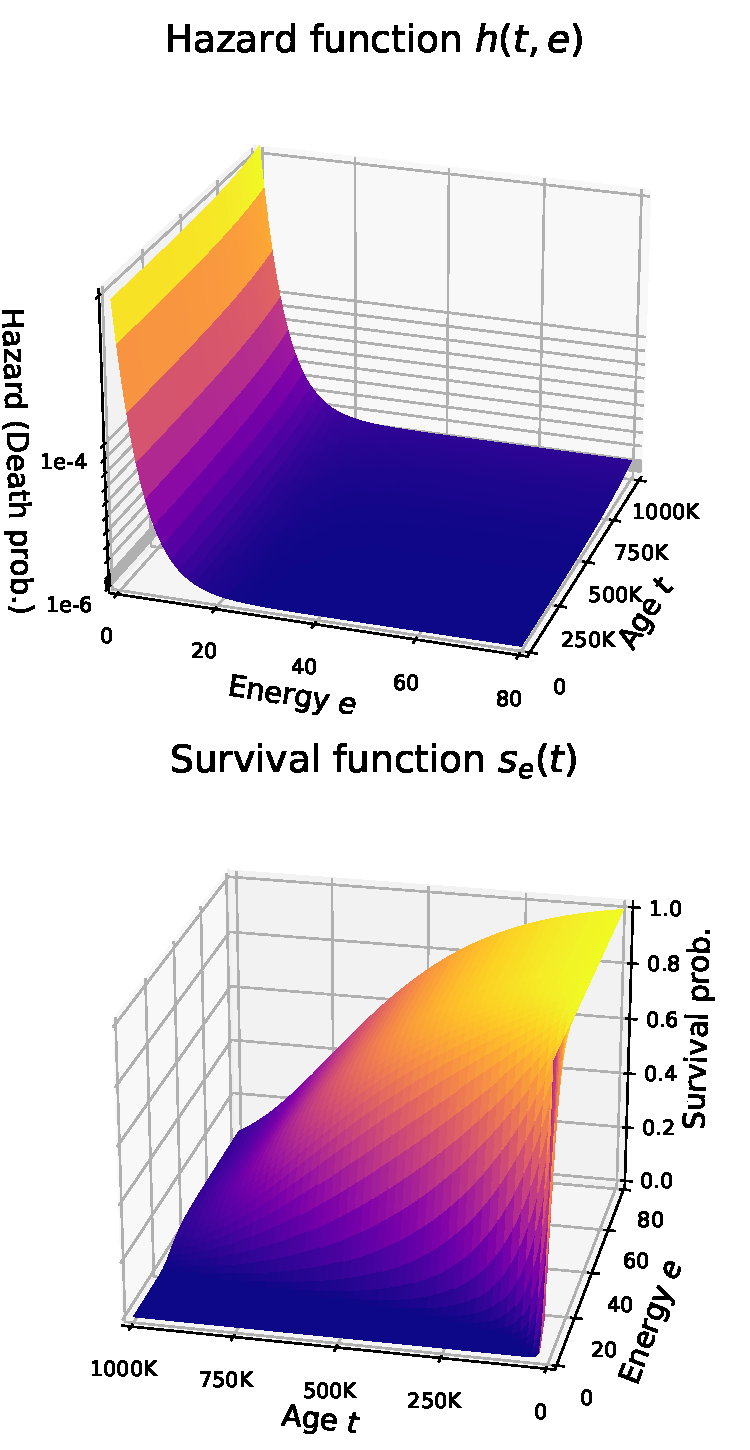
\includegraphics[width=15cm]{hazard_and_survival.pdf}
  \caption{
    \textbf{Left:} Designed hazard function $h(t)$ used for RL agents.
    \textbf{Right:} Survival function $S(t)$ corresponding to the hazard function.
  }\label{figure:hs}
\end{figure}

\paragraph{Energy-based death and birth model}
As a simple, but biologically-plausible way of simulating birth and death of agents, we employ an energy-based model similar to \citet{hamonEcoevolutionaryDynamicsNonepisodic2023}. Each agent maintains their own energy level $e$. Energy level $e$ increases by eating, and decreases by basic metabolism and taking an action in the environment. We design the agent's death and birth model so that maintaining higher energy level $e$ leads to longer lives and many offsprings. With $e$ and an agent's age $t$, we let $h(t, e)$ be the hazard function for agents that evaluates the probability for an agent to die:

\begin{align}
  h(t, e) = \kappa_{h} \left(1 - \frac{1}{1 + \alpha_{he} \exp(d_{h} - e)} \right) + \alpha_{ht} \exp(\beta t). \label{eq:h}
\end{align}

This hazard function\label{eq:h} consists of two terms. The first term increases as energy levels decrease follows a sigmoidal curve, where $\kappa_{h}, d_{h}$, and $\alpha_{he}$ are hyper parameters. The latter term $\alpha_{ht} \exp(\beta t)$ exponentially increases when the agent gets older, where $\alpha_{ht}$ and $\beta$ are hyper parameters. This is called Gompertz hazard model\citep{gompertzXXIVNatureFunction1825,kirkwoodDecipheringDeathCommentary2015} in population statistics. The left figure in \cref{figure:hs} shows the shape of hazard function with the specific parameters used in our experiments. To intuitively understand the behavior $h$, we plot survival function $S(t, e) = \exp (-\int_{0}^{t}(h(t, e)) dt)$ in the right of \cref{figure:hs}. $S(t, e)$ is the probability for an agent to survive to the age $t$ if it keeps the same energy level $e$. We can see that the survival probability more sharply decays with aging when the energy level is low.

\begin{figure}[t]
  \centering{}
  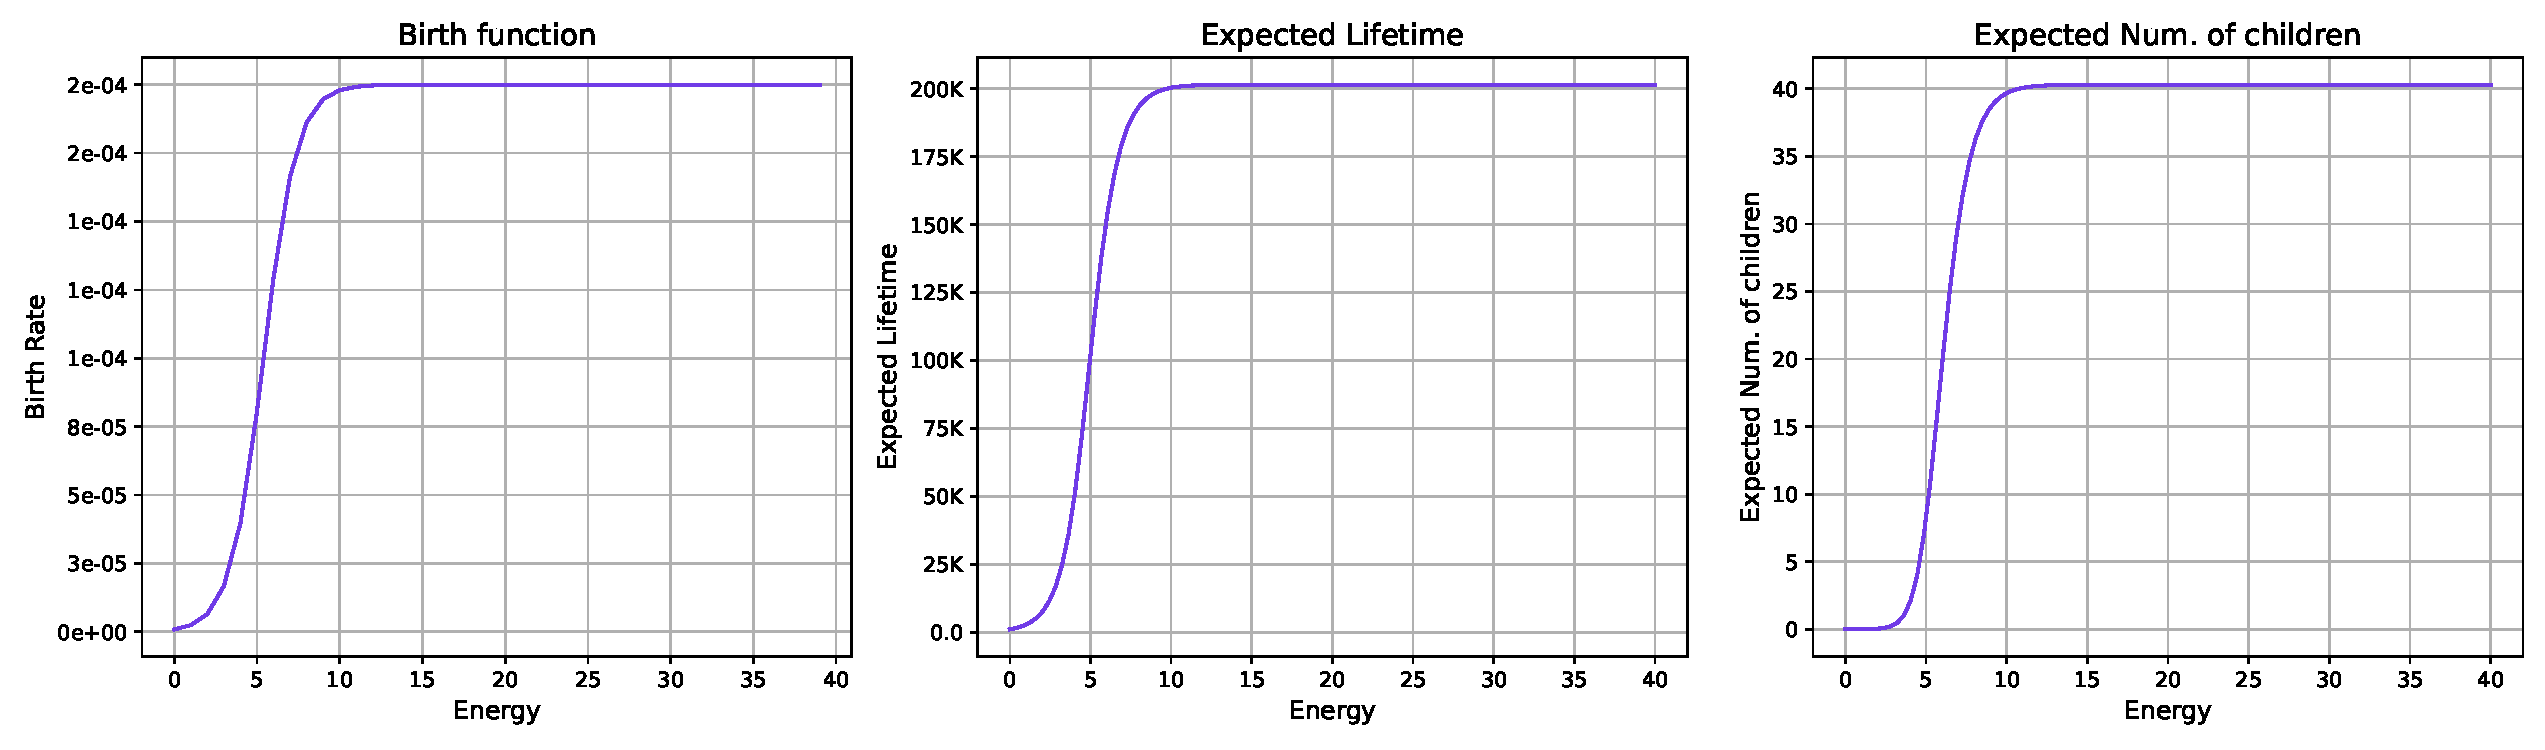
\includegraphics[width=15cm]{birth_and_nc.pdf}
  \caption{
    \textbf{Left:} Designed birth rate $b(e)$ for RL agents.
    \textbf{Center:} Expected lifetime for each agent
    \textbf{Right:} Expected reproduction number $R$ for RL agents corresponding to the designed hazard and birth functions.
  }\label{figure:bnc}
\end{figure}

For simplicity, we employ an asexual reproduction model where all agents can have a chance to make their children. We let $b(e)$ the birth function that evaluates the probability for an agent with energy level $e$ to make its own child. Similarly to the first term of \cref{eq:h}, we design the birth function $b$ as:
\begin{align}
 b(e) &=  \frac{\kappa_{b}}{1 + \alpha_{b}\exp(d_{b} - e)}. \label{eq:b}
\end{align}
Modeled as a generalized logistic function \citep{richardsFlexibleGrowthFunction1959}, $b(e)$ increases with $e$ following a sigmoidal curve where $\kappa_{b}$ is the scale, $d_{b}$ controls the delay of reaction, and $\alpha_{e}$ defines the shape of when $e=d_{b}$. The left figure of \cref{figure:bnc} shows the shape of $b$. For chosen $b$ and $h$, we plot the expected lifetime and expected number of children when an agent keeps the same energy level in the center and right figure in \cref{figure:bnc}. Parameters are chosen so that maximum expected lifetime is around \num{200000} and maximum expected number of children is around 40. All parameters used in experiments are are shown in \cref{ap:param}.

\paragraph{Environment}

\begin{figure}[t]
  \begin{subfigure}[t]{6cm}
    \centering
    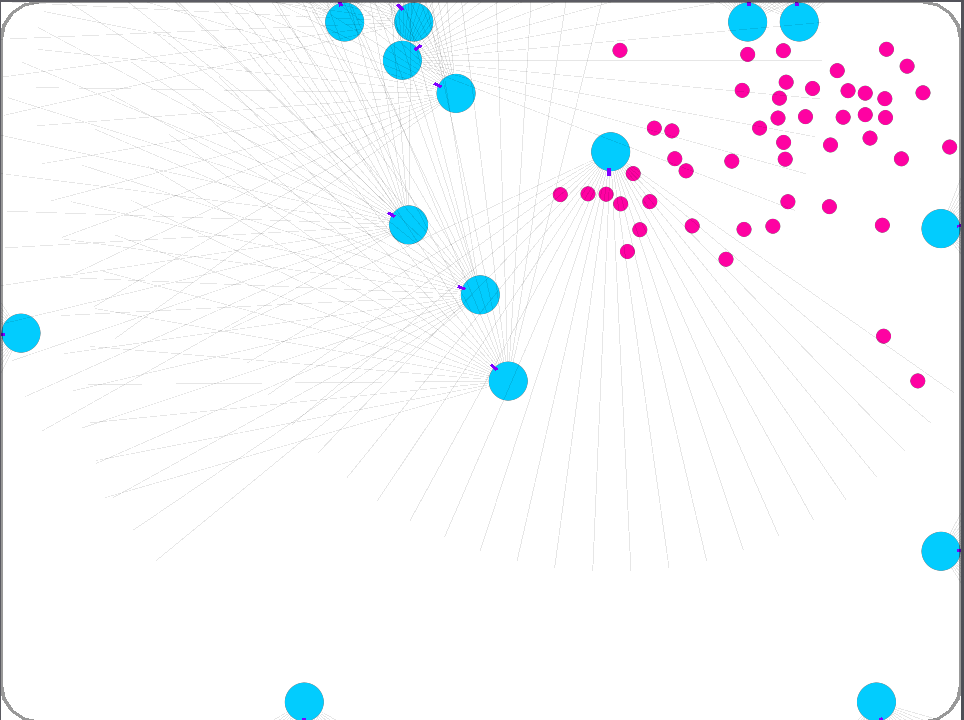
\includegraphics[width=6cm]{emevo-ss.png}
  \end{subfigure}
  \begin{subfigure}[t]{8cm}
    \centering
    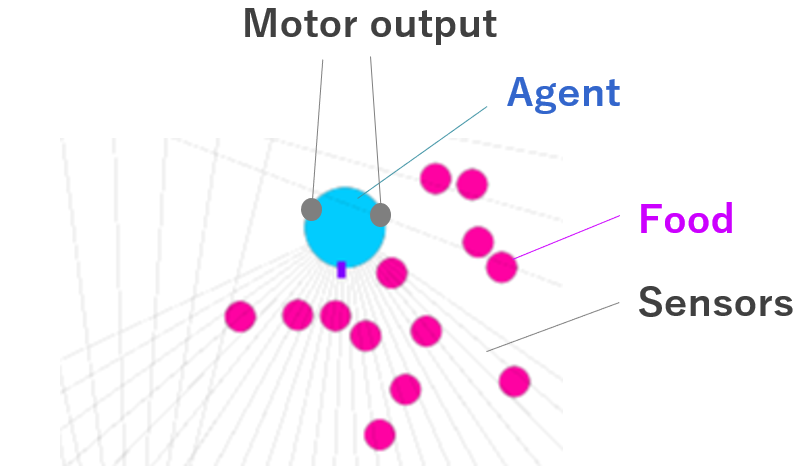
\includegraphics[width=8cm]{emevo-anno.png}
  \end{subfigure}
  \caption{
    \textbf{Left:} Environment.
    \textbf{Right:} Annotation
  }\label{figure:env}
\end{figure}

As a simple simulation environment yet with biologically-plausible sensorimotor interaction, we design a continuous 2D environment shown in \cref{figure:env}. Blue circles indicate agents and red circles indicate food. The environment is implemented by a two-dimensional rigid-body physics simulation, and agents can move by adding motor outputs at two points in the diagonal back part of the circle. An agent can eat food by touching it. After eaten, foods are regenerated in a random place. The rate of food regeneration follows logistic growth function $\frac{dN_{food}}{dt} = r N_{food} (1 - \frac{N_{food}}{N_{food}^{\mathrm{max}}}$, where $N_{food}$ is the number of food, $r$ is growth rate, and $N_{food}^{\mathrm{max}}$ is the maximum number of food. Eating food increases

When an agent makes a child, a new agent is placed in a random location sampled from a Gaussian distribution centered around its parent. The new agent inherits its reward function from its parent with some mutation, as described later. To avoid overlapping objects, we sample multiple random locations at one time, and choose one that does not conflict with any other object. However, to speed up simulation, reproduction just fails when all sampled locations are not available. Thus, keeping away from other agents is beneficial for agents to make more children. When an agent dies, its body is immediately removed from the environment.

Simulating many agents to maintain a reasonable size population (e.g., $50\sim 100$) is key in our evolution scheme. However, in our preliminary experiments used CPU-based simulation, we found that simulating collisions between many agents and foods could be a huge bottleneck in computation time. To overcome this challenge, we implement our environment using JAX Python library \citep{jax2018github} so that it can work on hardware accelerators such as GPU. Inspired by recent works on 3D rigid body physics simulation using JAX (e.g., \citet{brax2021github} and MuJoCo \citep{todorov2012mujoco} MJX\footnote{\url{https://mujoco.readthedocs.io/en/stable/mjx.html}}), we implement our own 2D physics engine using JAX and build our environment on top of that. This design decision is made because many of existing JAX-based physics simulation libraries are optimized for single-agent robot control and not well suited for handling multi-agent scenario we are dealing with. We explain implementation detail in \cref{ap:phys}.

\paragraph{Reward Model}

As a reward function, we used a simple linear function $\mathbf{r} = \left(r_{\textrm{agent}}, r_{\textrm{food}}, r_{\textrm{wall}}, r_{\textrm{action}} \right)^{\intercal} $ for an agent's collision and action. Let $c_{t}^{\textrm{agent}}, c_{t}^{\textrm{food}}$, and $c_{t}^{\textrm{wall}}$ be binary variables representing the agent's collision with other agents, food, and walls and obstacles at time $t$. In addition, let $J_{t}^{\textrm{norm}} = \frac{|J_{t}|}{\max{|J|}}$ denote the $[0, 1]-$normalized impulse an agent adds to itself at time $t$. Then, $\mathbf{r}$ maps these four values to a single scalar reward by $r = \mathbf{r}^{\intercal} (c_{t}^{\textrm{agent}}, c_{t}^{\textrm{food}}, c_{t}^{\textrm{wall}}, J_{t}^{\textrm{norm}})^{\intercal}$. $\mathbf{r}$ is the only genetically inheritable trait for the agent, with noise added by mutation at a certain probability. I may use a more complex reward function in future experiments, but for this preliminary experiment, I preferred simplicity. Mutation gives noise sampled from a mixture of binominal and Gaussian distribution. Specifically, uniform noise $[-0.1, 0.1]$ is added with probability $0.4$ to each element of $\mathbf{r}$.

I assume that each agent already knows how to learn from rewards. I used PPO\citep{schulmanProximalPolicyOptimization2017} as an RL algorithm because of its fast simulation performance. To estimate $A^{\pi}$, GAE (\cref{eq:gae}) is used with $N=1024$, so an agent learns only once every $1024$ step. As a neural network function approximation, I used a simple linear network shown by \cref{eq:v-nn} with additional layers for modeling $\pi$. Following the common practice in the literature, I modeled $\pi(\cdot|\textbf{s})$ as independent Gaussian distributions for each $ (J, \theta_{J}, \frac{d\theta_{\textrm{ang}}}{dt}) $ with state-independent variance. Other RL-related parameters are put in \cref{tab:rl-param}.

$r = r_{\textrm{agent}}c_{t}^{\textrm{agent}} + r_{\textrm{food}}c_{t}^{\textrm{food}} + r_{\textrm{wall}}c_{t}^{\textrm{wall}} + r_{\textrm{action}}J_{t}^{\textrm{norm}}$

\begin{algorithm}
  \caption{Pseudo code of reward evolution with asexual reproduction}\label{alg:reward-evo}
  \begin{tabular}{lll}
    \textbf{Input:} & $Pop$ & Initial population \\
                    & $Env$ & Simulated environment \\
                    & $N$ & Number of rollout steps used in RL \\
                    & $h(s, e)$ & Hazard function for agents \\
                    & $b(e)$ & Birth function for agents \\
  \end{tabular}
  \begin{algorithmic}[1]
    \Loop{}
    \ForAll{$agent \in Pop$}
      \State{$s \gets agent$'s observation in $Env$}
      \State{Sample an action $a$ from $agent$'s policy $\pi_{agent}(\cdot|s)$}
      \State{Update $agent$'s energy level $e$ based on the taken action $a$ and eaten food}
      \Once{in $N$ steps}
        \State{Update $agent$'s policy $\pi_{agent}$ and value function $\vh_{agent}$ via RL}
      \EndOnce{}
    \EndFor{}

    \State{Step the simulated environment $Env$ one step using collected actions}
    \LComment{Process death and birth}
    \ForAll{$agent \in Pop$ whose energy level is $e$ and age is $t$}
      \With{Probability $h(s, e)$}
        \State{$agent$ is removed from $Pop$ and $Env$}
        \Comment{agent is dead}
      \EndWith{}
      \With{Probability $b(e)$}
        \State{$\mathbf{r}_{\textrm{new}} \gets$ $agent$'s $\mathbf{r}~ + $ sampled noise}
        \State{Add a new agent with $\mathbf{r}_{\textrm{new}}$ to $Pop$ and $Env$}
      \EndWith{}
    \EndFor{}
  \EndLoop{}
\end{algorithmic}
\end{algorithm}

To summarize, I show the whole simulation process of reward evolution with asexual reproduction \Cref{alg:reward-evo}. Sexual reproduction may be considered in future studies, but only asexual reproduction was considered in this preliminary experiment. Basically, each agent acts based on their policy, and they occasionally update their policy via RL. They consume energy by acting and learning but can get energy by eating food. At each simulation step, an agent dies with probability $h(t, e)$ and creates a child with probability $b(e)$. The new agent inherits the reward function of its parent but may also acquire a new one via mutation. The implementation is done via Jax framework (e.g., \citet{jax2018github} and MuJoCo) in Python to benefit from vectorization on both CPU and GPU. Further thread-level parallelization may be considered in future research.

\section{Results}

\section{Conclusion}